\documentclass[16pt]{beamer}
\usepackage[utf8]{inputenc}

\title{Le réseau qui m'aimait}

\usetheme{default}

\usepackage[utf8]{inputenc}
\usepackage{amsmath}
\usepackage{amsfonts}
\usepackage{amssymb}
\usepackage{pgf}
\usepackage{color}
\usepackage[frenchb]{babel}
\usepackage{amssymb}
\usepackage{hyperref}

\usefonttheme{default}
\usepackage{DejaVuSans}
%\usepackage[sfdefault]{FiraSans} %% option 'sfdefault' activates Fira Sans as the default text font
\usepackage[T1]{fontenc}
\renewcommand*\oldstylenums[1]{{\firaoldstyle #1}}


\setbeamertemplate{navigation symbols}{} %remove navigation symbols

\author{Cédric Jeanneret (aka \href{https://www.twitter.com/SwissTengu}{@SwissTengu})}
\institute{\href{https://www.ethack.org/}{EthACK.org}}
\date{\today}

\definecolor{linecolor}{HTML}{4d4c4c}

\setbeamercolor{linecolor}{fg=white,bg=linecolor}

\setbeamertemplate{headline} {
	\begin{beamercolorbox}[wd=\paperwidth,dp=8pt,ht=12pt,leftskip=.29cm,rightskip=.29cm]{linecolor}
	\hfill
	\hypersetup{
		colorlinks=true,
		linkcolor=white,
		urlcolor=white,
	}
	\insertinstitute
	\end{beamercolorbox}%
}

\setbeamertemplate{footline}{%
	\begin{beamercolorbox}[wd=\paperwidth,dp=9pt,ht=0.4cm,leftskip=.29cm,rightskip=.3cm]{linecolor}
	\pgfputat{\pgfxy(0.455,-0.315)}{\pgfbox[center,base]{
\includegraphics[width=1.5cm]{../common/logo_537.png}}}
	\hfill
	\inserttitle
	\end{beamercolorbox}%
}


\hypersetup{
	colorlinks=true,
	linkcolor=blue,
	urlcolor=blue,
	pdfborderstyle={/S/U/W 1},
	pdfborder=0 0 1,
	linkbordercolor={0 0 0},
	urlbordercolor={0 0 0},
}


\begin{document}

{
\setbeamertemplate{footline}{%
	\begin{beamercolorbox}[wd=\paperwidth,dp=8pt,ht=12pt,leftskip=.29cm,rightskip=.3cm]{linecolor}
	\hfill
	\inserttitle
	\end{beamercolorbox}%
}

% center first slide — not a title, but almost
{
\centering
\begin{frame}

EthACK
\vspace{0.5cm}

The Swiss Privacy Basecamp 
\vspace{0.5cm}


\includegraphics[width=4cm]{../common/logo_537.png}

\end{frame}
}
}

\begin{frame}{EthACK ?}
\begin{itemize}
	\item Éthique
	\item État
	\item ACKnowledgement (reconnaissance)
	\item Hacking (éthique, évidemment)
	\item …
\end{itemize}
\end{frame}

\begin{frame}{Pourquoi ?}
\begin{itemize}
	\item Notre gouvernement ne s'intéresse pas (ou peu) au sujet
	\item Les sociétés privées nous fichent à notre insu
	\item Personne ne sait où sont leurs données, qui les traitent, à quoi elles servent
\end{itemize}
\end{frame}


\begin{frame}
  \titlepage
\end{frame}

\begin{frame}
{Déroulement}
\begin{itemize}
\item Ce que vous donnez de plein gré
\item Ce qui est collecté "en plus"
\item Buts avoués
\item Ce qu'on ne vous dit pas
\end{itemize}
\end{frame}

\begin{frame}
{Vos données personnelles}
\begin{itemize}
\item Nom, prénom
\item Âge
\item Pays, voire ville, voire…
\end{itemize}
\end{frame}

\begin{frame}
{Qui d'autre peut le savoir ?}
\onslide<+->{}
\begin{itemize}
\item<+-> Ceux qui lisent le bottin et actes de naissance
\item<+-> Le gouvernement
\item<+-> Vos amis et proches
\end{itemize}
\end{frame}

\begin{frame}
{Connexions}
\begin{itemize}
\item Vos liens de parenté
\item Vos amis
\item Vos connaissances
\end{itemize}
\end{frame}

\begin{frame}
{Qui d'autre peut le savoir ?}
\onslide<+->{}
\begin{itemize}
\item<+-> Le gouvernement
\item<+-> Vos amis et proches
\end{itemize}
\end{frame}

\begin{frame}
{Autres données}
\begin{itemize}
\item Vos photos de soirées
\item Votre localisation GPS
\item Votre état d'esprit par l'analyse de vos écrits
\end{itemize}
\end{frame}

\begin{frame}
{Qui d'autre peut le savoir ?}
\centering
Bah personne ne peut avoir tout cela.\newline
\vspace{1cm}
\newline
… À part vous-même !
\end{frame}

\begin{frame}
\centering

\includegraphics[width=\textwidth,keepaspectratio]{./you_cant_be_serious.jpg}
\end{frame}

\begin{frame}
{Ce qui est collecté en plus}
\centering
Parce qu'évidemment, vous ne donnerez pas tout.\newline
\vspace{1cm}
\newline
Quoique… ?
\end{frame}

\begin{frame}
{Les photos de vos amis}
\begin{itemize}
\item On peut vous désigner sur une photo
\item Données exifs (geotags etc)
\item On peut faire cela dans votre dos
\end{itemize}
\end{frame}

\begin{frame}
{Tout le reste}
\begin{itemize}
\item Boutons "j'aime"
\item Jeux
\item<+-> Applications
\item<+-> … Vous êtes encore là ? ;)
\end{itemize}
\end{frame}

\begin{frame}
\centering

\includegraphics[width=\textwidth,keepaspectratio]{./lalalalala-I-cant-hear-you.jpg}
\end{frame}

\begin{frame}
{Mais pourquoi ?!}
\centering
Oui, pourquoi tout collecter, étendre, conserver, analyser ?
\end{frame}

\begin{frame}
{Ce qu'on vous dit en gras}
\centering
"Connect with friends and the world around you on Facebook."\newline
\vspace{2cm} \newline
\tiny{"Connectez-vous avec vos amis et votre monde sur Facebook."}
\end{frame}

\begin{frame}
{Business model}
\centering
La pub !
\end{frame}

\begin{frame}
\centering
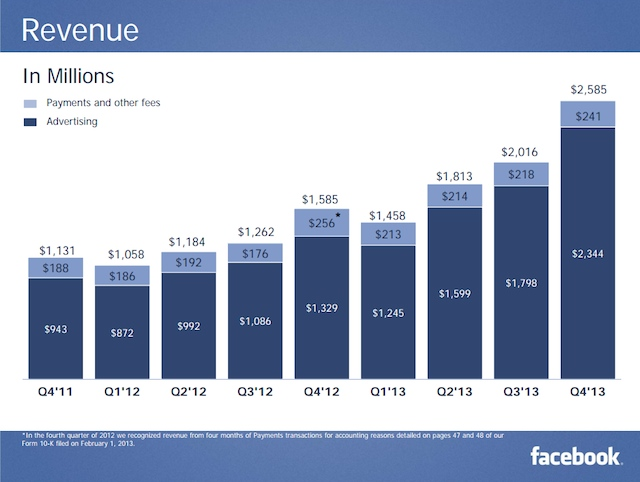
\includegraphics[height=\textheight,keepaspectratio]{./facebook-2013-q4-revenus.jpg}
\end{frame}

\begin{frame}
\centering
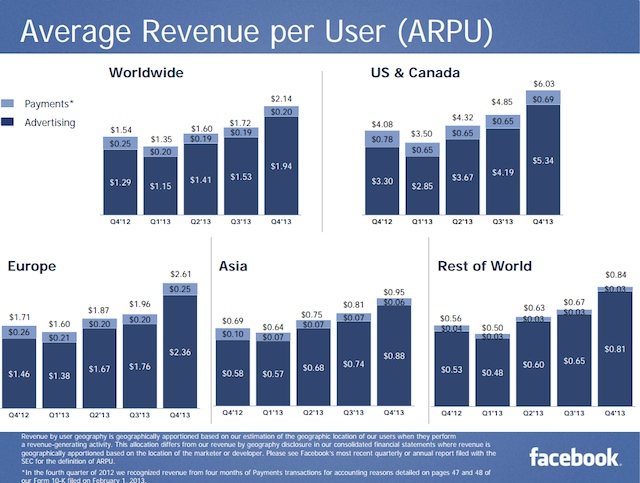
\includegraphics[height=\textheight,keepaspectratio]{./facebook-2013-q4-arpu.jpg}
\end{frame}

\begin{frame}
{Informations très précises sur vous}
\begin{itemize}
\item Vos goûts
\item Vos préférences
\item Vos habitudes
\item Celles de vos connaissances
\item Votre mentalité
\end{itemize}
\end{frame}

\begin{frame}

\includegraphics[width=\textwidth,keepaspectratio]{./Money-Money.jpg}
\end{frame}

\begin{frame}
{Et ce n'est pas fini}
\centering
On ne vous dit pas tout !
\end{frame}

\begin{frame}
{Mises à jour des CGU}
\begin{itemize}
\item Vous recevez un mail
\item Vous pouvez "discuter"
\item Facebook applique ce qu'il veut
\item Et modifie les règles de confidentialité à l'envi
\end{itemize}
\end{frame}

\begin{frame}
\centering

\includegraphics[height=\textheight,keepaspectratio]{./enough.png}
\end{frame}

\begin{frame}
{Je quitte Facebook !}
Cool, mais :
\begin{itemize}
\item Données conservées
\item Facebook parvient à les mettre à jour à votre insu
\end{itemize}
\end{frame}

\begin{frame}
{Je supprime mes photos !}
\centering
Facebook les conserve… Et les utilise encore\newline

\end{frame}

\begin{frame}
\centering

\includegraphics[width=\textwidth,keepaspectratio]{./kidding.jpeg}
\end{frame}

\begin{frame}
{
Nope…
}
you grant us a non-exclusive, transferable, sub-licensable, royalty-free, worldwide license to use any IP content that you post on or in connection with Facebook (IP License). This IP License ends when you delete your IP content or your account unless your content has been shared with others, and they have not deleted it.\newline
\vspace{0.5cm}\newline
\tiny{Extrait des \href{https://www.facebook.com/terms.php}{Terms of Service}}
\end{frame}

\begin{frame}
{L'aviez-vous lu ?}
\centering

\includegraphics[height=5cm,keepaspectratio]{./trollface1.jpg}
\end{frame}

\begin{frame}
{Que faire ?}
\centering

\includegraphics[height=5cm,keepaspectratio]{./doomed.jpg}
\end{frame}

\begin{frame}
{À part éviter Facebook…}
\begin{itemize}
\item Trier ce qu'on publie
\item Passer régulièrement dans les réglages
\item S'assurer qu'on a un droit de regard
\item Filtrer ses "amis"
\end{itemize}
\end{frame}

\begin{frame}
{Note pour les parents}
\begin{itemize}
\item Droit à l'image de l'enfant !
\item Pensez à son futur
\item \href{http://francoischarlet.ch/2013/parents-reflechissez-avant-de-publier-sur-internet-des-informations-sur-vos-enfants/}{Lisez cet article (francoischarlet.ch)}
\end{itemize}
\end{frame}

\begin{frame}
{Conclusion}
Facebook est "un" réseau parmi d'autres. N'oubliez pas que tout ce que vous publiez sur ces sites
est, par définition, public.
\end{frame}

{
\setbeamertemplate{footline}{%
	\begin{beamercolorbox}[wd=\paperwidth,dp=8pt,ht=12pt,leftskip=.29cm,rightskip=.3cm]{linecolor}
	\hfill
	\inserttitle
	\end{beamercolorbox}%
}
{
\centering
\begin{frame}
{Questions ?}

\href{https://ethack.org/}{https://ethack.org/} \\
\vspace{0.3cm}
\href{https://www.twitter.com/EthACK_org}{@EthACK\_org} on Twitter \\
\vspace{0.3cm}
\href{https://www.facebook.com/ethack.org}{ethack.org} on Facebook

\vspace{0.5cm}


\includegraphics[width=4cm]{../common/logo_537.png}
\end{frame}
}
}

\end{document}